% ----------------------------------------------------------------------------------------
%	Configuration
%----------------------------------------------------------------------------------------

\documentclass[aspectratio=169]{beamer}

\usetheme[titleformat=regular,numbering=none,progressbar=frametitle]{metropolis}

% newcastle colour scheme
\definecolor{nclBlue}{HTML}{003A65}
\definecolor{nclRed}{HTML}{D91A35}

\setbeamercovered{transparent}
\setbeamercovered{invisible}
\setbeamercolor{progress bar}{fg=nclRed}
\setbeamercolor{frametitle}{bg=nclBlue}
\setbeamercolor{background canvas}{bg=white}
\setbeamercolor{block body}{bg=gray!30}
\setbeamercolor{block title}{bg=nclBlue,fg=white}
\setbeamercolor{palette primary}{fg=white, bg=nclBlue}

\linespread{1.5}

\usepackage{graphicx}
\usepackage{booktabs}
\usepackage{amssymb}
\usepackage{pifont}
\usepackage{textcomp}
\usepackage{xcolor}
\usepackage{url}
\usepackage{amsmath}
\usepackage{mathspec}
\usepackage[font=footnotesize]{caption}

% Thin fonts
\setsansfont[BoldFont={Fira Sans}, Numbers={OldStyle}]{Fira Sans Light}
\setmathsfont(Digits)[Numbers={Lining, Proportional}]{Fira Sans Light}

% Thick fonts
% \setsansfont[BoldFont={Fira Sans SemiBold}, Numbers={OldStyle}]{Fira Sans}
% \setmathsfont(Digits)[Numbers={Lining, Proportional}]{Fira Sans Book}

% tikz configuration
\usetikzlibrary{shapes.geometric, arrows}
\usetikzlibrary{arrows, positioning, shapes}
\usetikzlibrary{decorations.pathmorphing}
\usetikzlibrary{calc}


\tikzstyle{vertex} = [circle, minimum width=15pt,draw,inner sep=0pt]
\tikzstyle{mini_vertex} = [circle, minimum width=15pt,draw,inner sep=0pt]
\tikzstyle{server} = [rectangle, rounded corners,minimum width=3cm,minimum height=4cm,draw=black]
\tikzstyle{mini_server} = [rectangle, rounded corners,minimum width=1.5cm,minimum height=1.9cm,draw=black]
\tikzstyle{local} = [thick,->,>=stealth]
\tikzstyle{dist} = [thick,dashed,->,>=stealth]
\tikzstyle{bignode}=[draw, circle, minimum width=70pt,align=center]

%----------------------------------------------------------------------------------------
%	Title + Overview Slide
% ----------------------------------------------------------------------------------------


\title[]{Design and Evaluation of an Edge Concurrency \\ Control Protocol for Distributed Graph Databases}

\author[Ezhilchelvan \& Mitrani \& Waudby \& Webber]{Paul Ezhilchelvan$^{1}$, Isi Mitrani$^{1}$, \underline{\emph{Jack Waudby}}$^{1}$ \& Jim Webber$^{2}$}
\institute[NCL]
{
  $^{1}$Newcastle University\\
  $^{2}$Neo4j
}
\date{November 28, 2019}

\begin{document}

\begin{frame}
\maketitle
\begin{tikzpicture}[overlay, remember picture]
  \node[above left=2.8cm and 0.852cm of current page.south east]{
\includegraphics[width=3cm]{images/logo_newcastle_uni.png}};
  \node[above left=1.2cm and 0.852cm of current page.south east]{
\includegraphics[width=3cm]{images/logo_neo4j.png}};
\end{tikzpicture}
\end{frame}


%----------------------------------------------------------------------------------------
%	PRESENTATION SLIDES
%----------------------------------------------------------------------------------------

%------------------------------------------------
% Background
% ------------------------------------------------

\setcounter{framenumber}{0}
\metroset{numbering=counter}


\begin{frame}
  \frametitle{Graph Databases}
    \begin{figure}
      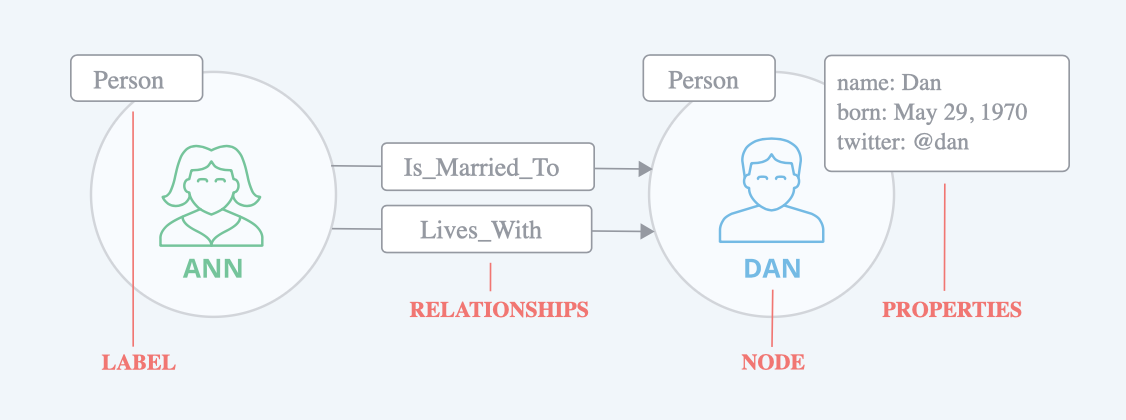
\includegraphics[scale=0.5]{images/property_graph.png}
      \caption{Labeled property graph\footnotemark}
    \end{figure}
  \footnotetext[1]{
    \url{https://neo4j.com}
  }
\end{frame}

% \begin{frame}
%   \frametitle{Graph Databases}
%     \begin{figure}
%       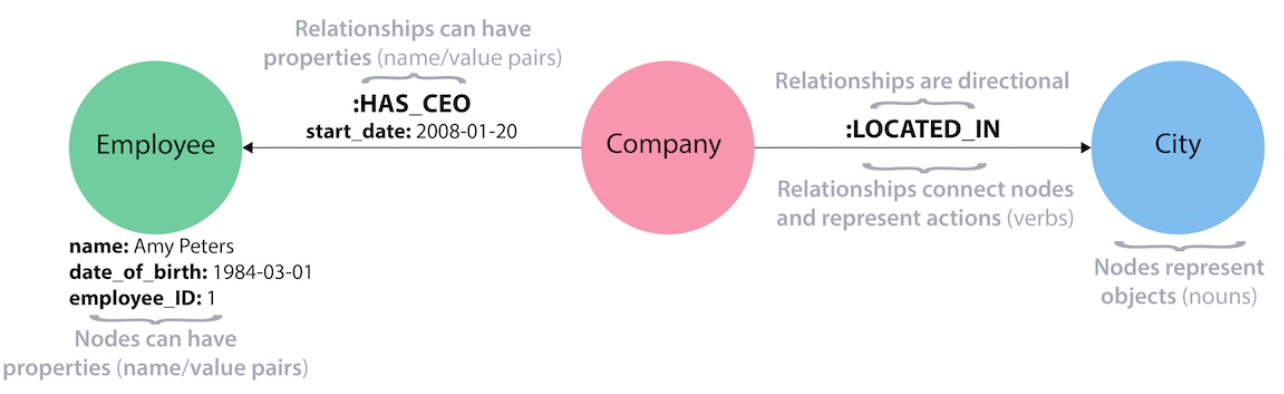
\includegraphics[scale=0.5]{images/property_graph_2.png}
%       \caption{Labeled property graph\footnotemark}
%     \end{figure}
%   \footnotetext[1]{
%     \url{https://neo4j.com}
%   }
% \end{frame}

\begin{frame}
  \frametitle{Graph Databases}
  \begin{itemize}
    \uncover<1->{
    \item \textbf{Efficient graph analysis:} reachability, pattern matching, shortest path search and clustering
    }
    \uncover<2->{
    \item \textbf{Use cases:} telecommunications, pharma, publishing, finance, social media
    }
  \end{itemize}
\end{frame}

\begin{frame}
  \frametitle{Graph Database Popularity}
  \begin{figure}[h!]
    \centering
    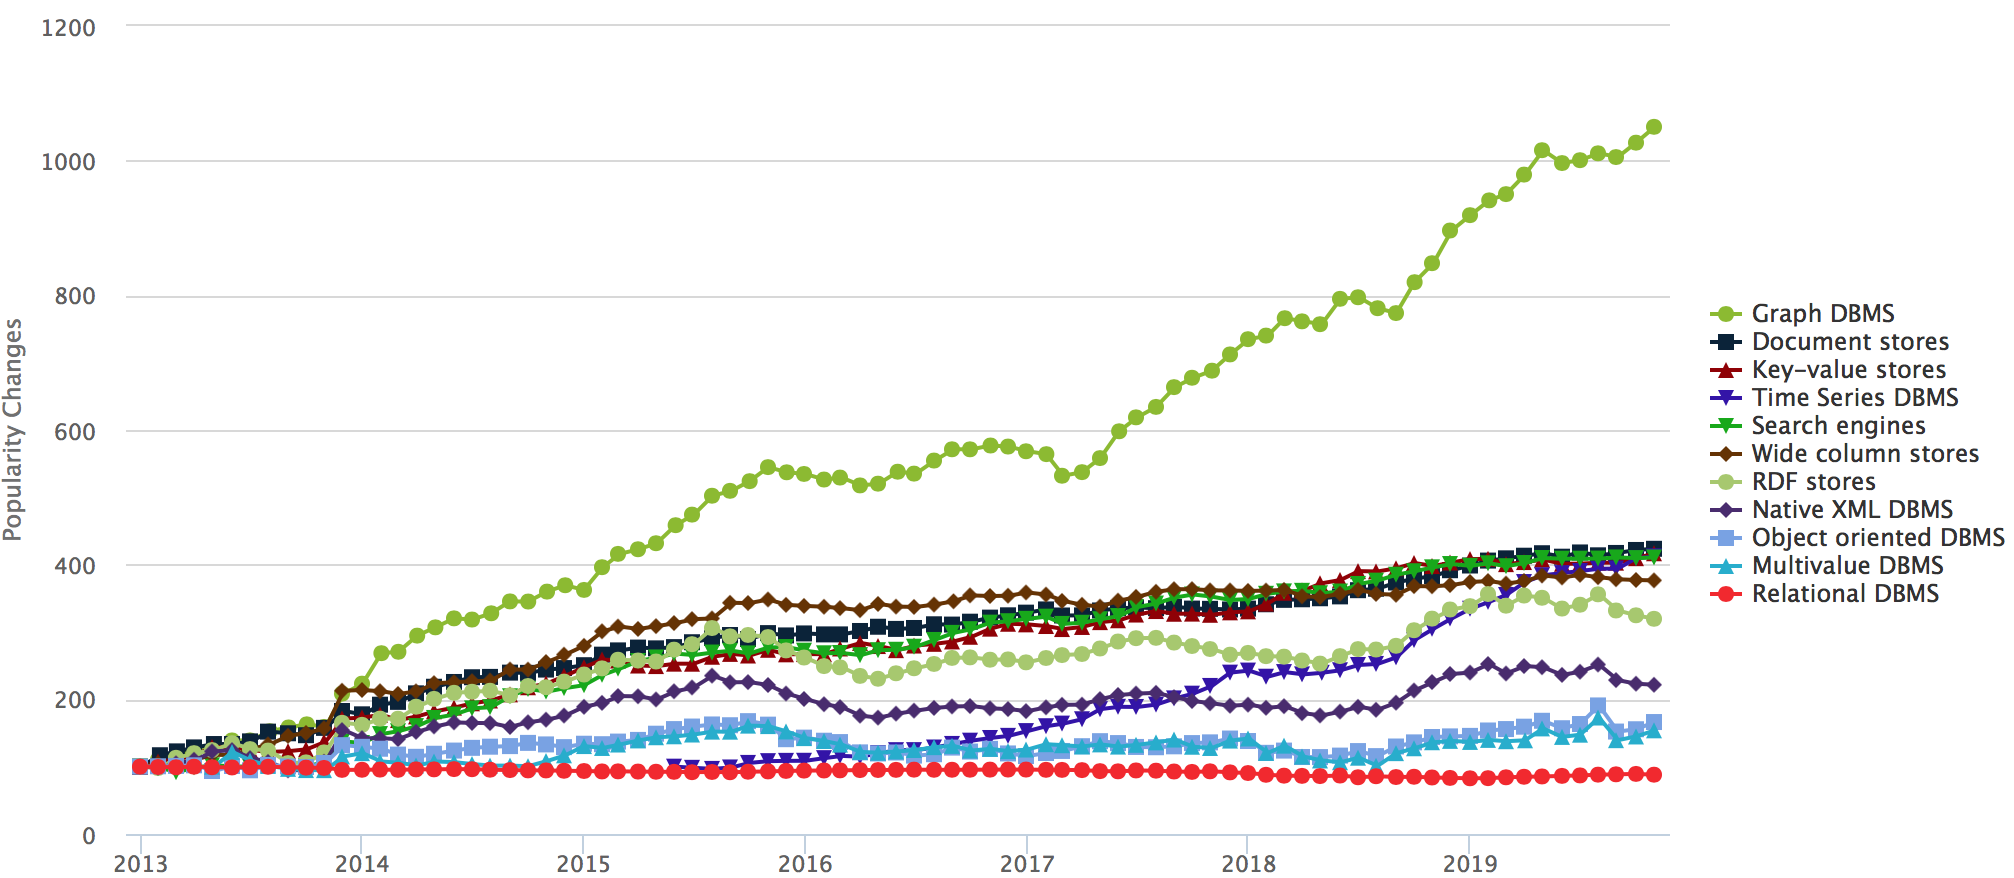
\includegraphics[scale=0.3]{images/db_popularity.png}
    \caption{Database popularity by data model\footnotemark}
  \end{figure}
  \footnotetext[1]{
    \url{https://db-engines.com/en/ranking_categories}
  }
\end{frame}

\begin{frame}
  \frametitle{Distributed Graph Databases}
  \begin{itemize}
    \uncover<1->{
    \item Graph exceeds the storage capacity of a single machine
    }
    \uncover<2->{
    \item Partition the graph across multiple machines in a cluster, with partitions replicated for fault-tolerance and availability
    }
    \uncover<3->{
    \item Graph partitioning inevitably leads to \textbf{distributed edges}
    }
  \end{itemize}
\end{frame}


\begin{frame}
  \frametitle{Distributed Graph Databases: Partitioning}
  \begin{figure}[h!]
    \centering
    \resizebox{0.6\textwidth}{!}{
    \begin{tikzpicture}[node distance=2cm]
      \node (v1) [vertex] {};
      \node (v2) [vertex, above of=v1,xshift=0.3cm] {};
      \node (v3) [vertex, above right of=v1,yshift=-0.3cm] {};
      \node (v4) [vertex, right of=v3,yshift=-0.3cm] {};
      \node (v5) [vertex, above left of=v4,xshift=0.7cm] {};
      \node (v6) [vertex, right of=v5,xshift=-0.8cm,yshift=1.2cm] {};
      \node (v7) [vertex, below right of=v6, yshift=-0.8cm] {};
      \node (v8) [vertex, below of=v7, yshift=0.3cm,xshift=0.3cm] {};
      \node (v9) [vertex, right of=v7,xshift=-0.4cm,yshift=0cm] {};
      \node (v10) [vertex, above left of=v9,xshift=0.4cm,yshift=-0.4cm] {};
      \node (v11) [vertex, above right of=v10,yshift=-2.5cm,xshift=1cm] {};
      \node (v12) [vertex, above of=v10,yshift=-0.6cm,xshift=1cm] {};
      \node (v13) [vertex, above right of=v6,yshift=-0.4cm,xshift=-0.1cm] {};
      \draw [local] (v2) -- (v1);
      \draw [local] (v1) -- (v3);
      \draw [local] (v3) -- (v2);
      \draw [local] (v2) -- (v5);
      \draw [local] (v1) -- (v4);
      \draw [local] (v5) -- (v4);
      \draw [local] (v5) -- (v6);
      \draw [local] (v4) -- (v7);
      \draw [local] (v8) -- (v4);
      \draw [local] (v8) -- (v9);
      \draw [local] (v9) -- (v11);
      \draw [local] (v10) -- (v7);
      \draw [local] (v10) -- (v12);
      \draw [local] (v12) -- (v13);
      \draw [local] (v10) -- (v6);
      \draw [local] (v10) -- (v11);
      \draw [local] (v13) -- (v10);
      \draw [local] (v11) -- (v12);
    \end{tikzpicture}
    }
    \caption{Connected graph}
  \end{figure}
\end{frame}

\begin{frame}
  \frametitle{Distributed Graph Databases: Partitioning}
  \begin{figure}[h!]
    \centering
    \resizebox{0.6\textwidth}{!}{
    \begin{tikzpicture}[node distance=2cm]
      \node (s1) [server,label=$S_1$] {};
      \node (s2) [server, right of=s1,xshift=2cm,yshift=2cm,label=$S_2$] {};
      \node (s3) [server, right of=s1,xshift=6cm,label=$S_3$] {};

      \node (v1) [vertex,xshift=-0.5cm,yshift=-1.5cm] {};
      \node (v2) [vertex, above of=v1,xshift=-0.3cm,yshift=1cm] {};
      \node (v3) [vertex, above of=v1,xshift=0.6cm] {};
      \node (v4) [vertex, below right of=v3,xshift=-0.5cm,yshift=-0.3cm] {};
      \node (v5) [vertex, above right of=v3,xshift=-0.6cm,yshift=-0.5cm] {};
      \node (v6) [vertex, right of=v5,xshift=0.3cm,yshift=0.8cm] {};
      \node (v7) [vertex, below of=v6, xshift=1cm,yshift=0.4cm] {};
      \node (v8) [vertex, right of=v4, yshift=-0.3cm,xshift=4.5cm] {};
      \node (v9) [vertex, above of=v8,xshift=-0.4cm,yshift=-0.5cm] {};
      \node (v10) [vertex, above of=v9,xshift=-2.5cm,yshift=-0.3cm] {};
      \node (v11) [vertex, right of=v9,yshift=0.5cm,xshift=-0.3cm] {};
      \node (v12) [vertex, above of=v11,yshift=-1cm,xshift=-1cm] {};
      \node (v13) [vertex, above right of=v6,yshift=-0.4cm,xshift=-0.1cm] {};
      \draw [local] (v2) -- (v1);
      \draw [local] (v1) -- (v3);
      \draw [local] (v3) -- (v2);
      \draw [local] (v2) -- (v5);
      \draw [local] (v1) -- (v4);
      \draw [local] (v5) -- (v4);
      \draw [dist] (v5) -- (v6);
      \draw [dist] (v4) -- (v7);
      \draw [dist] (v8) -- (v4);
      \draw [local] (v8) -- (v9);
      \draw [local] (v9) -- (v11);
      \draw [local] (v10) -- (v7);
      \draw [dist] (v10) -- (v12);
      \draw [dist] (v12) -- (v13);
      \draw [local] (v10) -- (v6);
      \draw [dist] (v10) -- (v11);
      \draw [local] (v13) -- (v10);
      \draw [local] (v11) -- (v12);
    \end{tikzpicture}
  }
\caption{Graph partitioned across 3 servers}
  \end{figure}
\end{frame}

%------------------------------------------------
% Problem 1: Reciprocal Consistency}
% ------------------------------------------------

\begin{frame}
  \frametitle{Reciprocal Consistency}
  \begin{center}
  \textbf{A logical edge is represented by 2 physical records}
  \end{center}
  \begin{figure}[h!]
    \centering
    \begin{tikzpicture}[node distance=7cm]
      \uncover<1-> {
      \node (n1) [bignode] {\texttt{Flight}};
      \node (rect)  [draw,dashed,minimum width=3cm,minimum height=3cm,label=above:{$S_1$}] {};
      \node (rect)  [draw,dashed,minimum width=3cm,minimum height=3cm,label,xshift=7cm,label=above:{$S_2$}] {};
      \node (n2) [bignode, right of=n1] {\texttt{Seat}};
      \draw [local] (n1) to[out=0,in=-180]  node[below] {\texttt{:AVAILABLE}} (n2);
    }
      \uncover<2-> {
         \node (q1) [rectangle, minimum width=0.6cm,minimum height=0.6cm,draw=black,xshift=0cm,yshift=-2.5cm] {\textit{Seat Available In Flight}};
         \node (q2) [rectangle,minimum width=0.6cm,minimum height=0.6cm,draw=black,xshift=7cm,yshift=-2.5cm] {\textit{Flight Has Seat Available}};
         \draw [<->,dashed](q1) -- (q2);
      }
    \end{tikzpicture}
    \caption{A reciprocal consistent edge}
  \end{figure}
\end{frame}


\begin{frame}
  \frametitle{Reciprocal Consistency Violation}
  Two concurrent transactions:
  \begin{itemize}
  \item Mr Red requests to book the seat, $T_R$
  \item Mr Blue requests to book the seat, $T_B$
  \end{itemize}
\end{frame}

\begin{frame}
  \frametitle{Reciprocal Consistency Violation}
  \begin{figure}[h!]
    \centering
    \begin{tikzpicture}[node distance=2cm]
      \uncover<1-> {
        \draw [black,<-,>=stealth] (0,0) -- (0,4) node [] {};
        \draw [black,<-,>=stealth] (4,0) -- (4,4) node [] {};
        \draw [black,dashed,->,>=stealth] (0,4.1) node [label=above:{$S_1$}] {} -- node [midway,above] {$E$} (4,4.1) node [label=above:{$S_2$}] {};
      }
      \uncover<2-3> {
        \draw [red,->,>=stealth] (0,3.6) node [label=left:{$T_R$}] {} -- (2,2.3);
      }
      \uncover<3-4> {
        \draw [blue,->,>=stealth] (4,3) node [label=right:{$T_B$}] {} -- (2,2.1);
      }
      \uncover<4-> {
        \draw [red,->,>=stealth] (0,3.6) node [label=left:{$T_R$}] {} -- (4,1);
      }
      \uncover<5-> {
        \draw [blue,->,>=stealth] (4,3) node [label=right:{$T_B$}] {} -- (0,1.2);
      }
    \end{tikzpicture}
    \caption{Concurrent transactions interleave and violate reciprocal consistency}
  \end{figure}
\end{frame}

\begin{frame}
  \frametitle{Reciprocal Consistency Violation}
  \begin{figure}[h!]
    \centering
    \begin{tikzpicture}[node distance=7cm]
      \node (n1) [bignode] {\texttt{Flight}};
      \node (rect)  [draw,dashed,minimum width=3cm,minimum height=3cm,label=above:{$S_1$}] {};
      \node (rect)  [draw,dashed,minimum width=3cm,minimum height=3cm,label,xshift=7cm,label=above:{$S_2$}] {};
      \node (n2) [bignode, right of=n1] {\texttt{Seat}};
      \draw [local] (n1) to[out=0,in=-180]  node[below] {\texttt{:BOOKED}} (n2);

      \uncover<2-> {
      \node (q1) [rectangle, minimum width=0.6cm,minimum height=0.6cm,draw=black,xshift=0cm,yshift=-2.5cm] {\textit{Mr Blue Booked In Seat}};
      \node (q2) [rectangle,minimum width=0.6cm,minimum height=0.6cm,draw=black,xshift=7cm,yshift=-2.5cm] {\textit{Mr Red Booked In Seat}};
      \draw [<->,dashed](q1) -- (q2);
      \draw [<->,dashed](q1) -- (q2);
      \coordinate (a) at (4,-2);
      \coordinate (b) at (3,-3);
      \coordinate (c) at (3,-2);
      \coordinate (d) at (4,-3);
      \draw [very thick,red] ($ (a) $) -- ($ (b) $);
      \draw [very thick,red] ($ (c) $) -- ($ (d) $);
    }
    \end{tikzpicture}
    \caption{Reciprocal inconsistent distributed edge}
  \end{figure}
\end{frame}

% \begin{frame}
%   \frametitle{Reciprocal Consistency Violation}
%   \begin{figure}[h!]
%     \centering
%     \begin{tikzpicture}[node distance=2cm]
%       \uncover<1->{
%         \draw [black,<-,>=stealth] (4.5,0) -- (4.5,4) node [] {};
%         \draw [red,->,>=stealth] (4.5,2.2) node [label=left:{$T_x$}] {} -- (6.5,1);
%         \draw [blue,->,>=stealth] (6.5,2.7) node [label=right:{$T_y$}] {} -- (4.5,1.2);
%         \draw [black,<-,>=stealth] (6.5,0) -- (6.5,4) node [] {};
%         \draw [black,dashed,->,>=stealth] (4.5,4.1) node [label=above:{$S_1$}] {} -- node [midway,above] {$E$} (6.5,4.1) node [label=above:{$S_2$}] {};
%       }
%       \uncover<2->{
%         \draw [black,<-,>=stealth] (9,0) -- (9,4) node [] {};
%         \draw [red,->,>=stealth] (9,3.5) node [label=left:{$T_x$}] {} -- (11,1);
%         \draw [blue,->,>=stealth] (9,2.8) node [label=left:{$T_y$}] {} -- (11,2);
%         \draw [black,<-,>=stealth] (11,0) -- (11,4) node [] {};
%         \draw [black,dashed,->,>=stealth] (9,4.1) node [label=above:{$S_1$}] {} -- node [midway,above] {$E$} (11,4.1) node [label=above:{$S_2$}] {};
%       }
%     \end{tikzpicture}
%     \caption{Possible interleaving of concurrent transactions that violate reciprocal consistency}
%   \end{figure}
% \end{frame}

\begin{frame}
  \frametitle{Distributed Edge Reciprocal Consistency}
  \begin{itemize}
    \uncover<1->{
  \item Without concurrency control, distributed edges can become reciprocally inconsistent
    \begin{itemize}
    \item A distributed edge's reciprocal information is separated by the network
    \end{itemize}
  }
  \uncover<2->{
  \item Reciprocal inconsistency is a source of corruption\footnotemark
  }
  \uncover<3->{
  \item No known concurrency control protocol exists specific to graph databases and maintaining reciprocal consistency
    }
    \end{itemize}
    \footnotetext[3]{Ezhilchelvan, P. et al, \textit{On the degradation of distributed graph databases with eventual consistency}. European Performance Engineering Workshop 2018.}
\end{frame}


\begin{frame}
  \frametitle{Our Solution: Collision Detection}
  \begin{itemize}
    \uncover<1->{
    \item Carefully abort transaction(s)
    }
    \uncover<2->{
    \item No centralized control or synchronized clock
    }
    \uncover<3->{
    \item Permits interleavings that preserve reciprocal consistency
    }
  \end{itemize}
\end{frame}

\begin{frame}
  \frametitle{Collision Detection General Rules}
  \begin{itemize}
    \uncover<1->{
    \item Updates are initially provisional
    }
    \uncover<2->{
    \item Transactions distinguish between their first and second updates using labels
    }
    \uncover<3->{
    \item When a transaction attempts to update a given record, it can identify all other transactions that have earlier updated that record provisionally
    }
  \end{itemize}
\end{frame}

\begin{frame}
  \frametitle{Interference-free Update}
  \begin{figure}[h!]
    \centering
    \begin{tikzpicture}
      \uncover<1->{
        \draw [black,<-,>=stealth] (-3,1) -- (-3,3) node [label=above:{time}] {};
        \draw [white,<-,>=stealth] (7,1) -- (7,3) ; %placeholder to balance picture
        \draw [black,<-,>=stealth] (0,0) -- (0,4) ;
        \draw [black,<-,>=stealth] (4,0) -- (4,4) ;
        \draw [black,dashed,->,>=stealth] (0,4.5) node [label=above:{$e_{out}$ in $S_1$}] {} -- (4,4.5) node [label=above:{$e_{in}$ in $S_2$}] {};
      }
      \uncover<2->{
        \node [] at (-0.5,4) {\textcolor{red}{$T_R$}};
      }
      \uncover<3->{
        \node [] at (-0.5,3.5) {\textcolor{red}{$1$}};
      }
      \uncover<3->{
        \draw [red,->,>=stealth] (0,3.5) node [] {} -- (4,0.3) node (TX) [] {};
      }
      \uncover<4->{
        \node [] at (4.5,0.3) {\textcolor{red}{$2$}};
      }
    \end{tikzpicture}
  \end{figure}

\end{frame}

\begin{frame}
  \frametitle{Collision Detection}
  \begin{center}
    \textbf{Rule: For any ``1'' seen, there must be a ``2'' in the opposite end. Else, abort}
  \end{center}
  \begin{figure}[h!]
    \centering
    \begin{tikzpicture}
      \uncover<2->{
        \draw [black,<-,>=stealth] (-3,1) -- (-3,3) node [label=above:{time}] {};
        \draw [black,<-,>=stealth] (0,0) -- (0,4) ;
        \draw [black,<-,>=stealth] (4,0) -- (4,4) ;
        \draw [black,dashed,->,>=stealth] (0,4.5) node [label=above:{$e_{out}$ in $S_1$}] {} -- (4,4.5) node [label=above:{$e_{in}$ in $S_2$}] {};
        \draw [white,<-,>=stealth] (7,1) -- (7,3) ; %placeholder to balance picture
      }
      \uncover<2->{
        \node [] at (-0.5,4) {\textcolor{red}{$T_R$}};
      }
      \uncover<3->{
        \node [] at (-0.5,3.5) {\textcolor{red}{$1$}};
      }
      \uncover<4-11>{
        \draw [red,->,>=stealth] (0,3.5) -- (2,1.9);
      }
      \uncover<5-10>{
        \node [] at (-0.5,2.6) {\textcolor{blue}{$T_B$}};
      }
      \uncover<6-10>{
        \node [] at (-0.5,2.1) {\textcolor{blue}{$1$}};
      }
      \uncover<7-7>{
        \draw [blue,->,>=stealth] (0,2.1) -- (2,1.8);
      }
      \uncover<8-10>{
        \draw [blue,->,>=stealth] (0,2.1) -- (4,1.5);
        \node [] at (4.5,1.5) {\textcolor{blue}{$2$}};
      }
      \uncover<9-9>{
        \node [] at (6,2) {$T_R$'s 2 is missing};
      }
      \uncover<10-10>{
        \node[] at (6,2) {$T_B$ ABORTS};
      }
      \uncover<12->{
        \draw [red,->,>=stealth] (0,3.5)  -- (4,0.3);
      }
      \uncover<13->{
        \node [] at (4.5,0.3) {\textcolor{red}{$2$}};
      }
      \uncover<14->{
        \node[] at (6,2) {$T_R$ SUCCEEDS};
        }
    \end{tikzpicture}
  \end{figure}
\end{frame}

%------------------------------------------------
%Problem 2: Edge-Order Consistency
% ------------------------------------------------

\begin{frame}
  \frametitle{Edge-Order Consistency}
  A second consistency problem related to distributed edges:
  \begin{itemize}
    \uncover<2->{
    \item Consider 2 transactions that update $2$ or more of the \textit{same} distributed edges
    }
    \uncover<3->{
    \item Each update is reciprocally consistent
    }
    \uncover<4->{
    \item Then if $T_R$ updates before $T_B$ on a given edge then this order should be preserved across all edges
    }
  \end{itemize}
\end{frame}

\begin{frame}
  \frametitle{Edge-Order Consistency Violation}
  Consider two edges,
  \begin{figure}[h!]
    \centering
    \resizebox{1\textwidth}{!}{
      \begin{tikzpicture}[node distance=5.2cm]
        \node[] at (2.6,2.5) {\large{$E$}};
        \node[] at (13,2.5) {\large{$E'$}};
        \node (n1) [bignode] {\texttt{Flight}};
        \node (rect)  [draw,dashed,minimum width=3cm,minimum height=3cm,label=above:{$S_1$}] {};
        \node (rect)  [draw,dashed,minimum width=3cm,minimum height=3cm,label,xshift=5.2cm,label=above:{$S_2$}] {};
        \node (n2) [bignode, right of=n1] {\texttt{Seat}};
        \draw [local] (n1) to[out=0,in=-180]  node[below] {\small{\texttt{:AVAILABLE}}} (n2);
        \node (q1) [rectangle, minimum width=0.6cm,minimum height=0.6cm,draw=black,xshift=0cm,yshift=-2cm] {\textit{Seat Available In Flight}};
        \node (q2) [rectangle,minimum width=0.6cm,minimum height=0.6cm,draw=black,xshift=5.2cm,yshift=-2cm] {\textit{In Flight Seat Available}};
         \draw [<->,dashed](q1) -- (q2);

        \node (n3) [bignode, right of=n2] {\texttt{Hotel}};
        \node (n4) [bignode, right of=n3] {\texttt{Room}};
        \draw [local] (n3) to[out=0,in=-180]  node[below] {\small{\texttt{:AVAILABLE}}} (n4);
        \node (q3) [rectangle, minimum width=0.6cm,minimum height=0.6cm,draw=black,xshift=10.4cm,yshift=-2cm] {\textit{Room Available In Hotel}};
        \node (q4) [rectangle,minimum width=0.6cm,minimum height=0.6cm,draw=black,xshift=15.6cm,yshift=-2cm] {\textit{In Hotel Room Available}};
        \node (rect)  [draw,dashed,minimum width=3cm,minimum height=3cm,xshift=15.6cm,label=above:{$S_4$}] {};
        \node (rect)  [draw,dashed,minimum width=3cm,minimum height=3cm,label,xshift=10.4cm,label=above:{$S_3$}] {};
        \draw [<->,dashed](q3) -- (q4);

      \end{tikzpicture}
    }
    \caption{Two distributed edges}
  \end{figure}
\end{frame}

\begin{frame}
  \frametitle{Edge-Order Consistency Violation}
  Two concurrent transactions by a travel agent:
  \begin{itemize}
  \item Requests to book room and seat for Mr Red, $T_R$
  \item Requests to book room and seat for Mr Blue, $T_B$
  \end{itemize}
\end{frame}

\begin{frame}
  \frametitle{Edge-Order Consistency Violation}
  \begin{figure}[h!]
    \centering
    \begin{tikzpicture}
      \uncover<1->{

        \draw [black,->,>=stealth] (0,0) -- (10,0) node [label=below:{$time$}] {};
        \draw [black,-,>=stealth] (2,4) node [label={[red]left:{$T_R$}}] {} -- (8,4);
        \draw [black,-,>=stealth] (8,4.1) node [] {} -- (8,3.9);
        \draw [black,-,>=stealth] (2,4.1) node [] {} -- (2,3.9);
        \draw [black,-,>=stealth] (4,2) node [label={[blue]left:{$T_B$}}] {} -- (7,2);
        \draw [black,-,>=stealth] (4,2.1) node [] {} -- (4,1.9);
        \draw [black,-,>=stealth] (7,2.1) node [] {} -- (7,1.9);
      }
      \uncover<2->{
        \draw [black,dashed] (2.5,0) node [label=below:{$t_1$}] {} -- (2.5,4) node [label=above:{$E$}] {};
      }
      \uncover<3->{
        \draw [black,dashed] (4.5,0) node [label=below:{$t_2$}] {} -- (4.5,2) node [label=above:{$E$}] {};
      }
      \uncover<4->{

        \draw [black,dashed] (6.5,0) node [label=below:{$t_3$}] {} -- (6.5,2) node [label=above:{$E'$}] {};
      }
      \uncover<5->{

        \draw [black,dashed] (7.5,0) node [label=below:{$t_4$}] {} -- (7.5,4) node [label=above:{$E'$}] {};
      }
      \uncover<6->{
        \draw (8.3,2) node [label=right:{$E : T_R \rightarrow T_B$}] {} ;
        \draw (8.3,1.5) node [label=right:{$E' : T_B \rightarrow T_R$}] {} ;
        \draw (8.3,1) rectangle (11,2.5);
      }
    \end{tikzpicture}
    \caption{Edge-order consistency violation}
  \end{figure}
\end{frame}

\begin{frame}
  \frametitle{Edge-Order Consistency Violation}
  \begin{figure}[h!]
    \centering
    \resizebox{1\textwidth}{!}{
      \begin{tikzpicture}[node distance=5cm]
        % edge labels
        \node[] at (2.5,3) {\large{$E$}};
        \node[] at (12.5,3) {\large{$E'$}};
        % edge 1: flight -> seat
        \node (n1) [bignode] {\texttt{Flight}};
        \node (n2) [bignode, right of=n1] {\texttt{Seat}};
        % edge 1: servers
        \node (rect)  [draw,dashed,minimum width=3cm,minimum height=3cm,label=above:{$S_1$}] {};
        \node (rect)  [draw,dashed,minimum width=3cm,minimum height=3cm,label,xshift=5cm,label=above:{$S_2$}] {};
        % edge 1
        \draw [local] (n1) to[out=0,in=-180]  node[below] {\texttt{:BOOKED}} (n2);
        % edge 1 information
        \node (q1) [rectangle, minimum width=0.6cm,minimum height=0.6cm,draw=black,xshift=0cm,yshift=-2cm] {\textcolor{red}{\textit{Mr Red Booked Seat}}};
        \node (q2) [rectangle,minimum width=0.6cm,minimum height=0.6cm,draw=black,xshift=5cm,yshift=-2cm] {\textcolor{red}{\textit{Mr Red Booked Seat}}};
        \draw [<->,dashed](q1) -- (q2);

        % edge 2: hotel -> room
        \node (n3) [bignode, right of=n2] {\texttt{Hotel}};
        \node (n4) [bignode, right of=n3] {\texttt{Room}};
        \draw [local] (n3) to[out=0,in=-180]  node[below] {\texttt{:BOOKED}} (n4);
        \node (q3) [rectangle, minimum width=0.6cm,minimum height=0.6cm,draw=black,xshift=10cm,yshift=-2cm] {\textcolor{blue}{\textit{Mr Blue Booked Room}}};
        \node (q4) [rectangle,minimum width=0.6cm,minimum height=0.6cm,draw=black,xshift=15cm,yshift=-2cm] {\textcolor{blue}{\textit{Mr Blue Booked Room}}};
        \node (rect)  [draw,dashed,minimum width=3cm,minimum height=3cm,xshift=15cm,label=above:{$S_4$}] {};
        \node (rect)  [draw,dashed,minimum width=3cm,minimum height=3cm,label,xshift=10cm,label=above:{$S_3$}] {};
        \draw [<->,dashed](q3) -- (q4);

      \end{tikzpicture}
    }
    \caption{Edge-order consistency violation}
  \end{figure}
\end{frame}

\begin{frame}
  \frametitle{Our Solution: Order Arbitration}
  \begin{itemize}
  \uncover<1->{
  \item Transactions collect predecessors from each update
  }
  \uncover<2->{
  \item Centralized arbiter maintains some global state
  }
  \uncover<3->{
  \item Global state used to detect edge-order violations
  }
  \uncover<4->{
  \item Offending transactions are aborted
  }
  \end{itemize}
\end{frame}

\begin{frame}
  \frametitle{Order Arbitration}
    \begin{center}
      \textbf{Rule: Collect predecessors after every successful update}
    \end{center}
  \begin{figure}[h!]
    \centering
    \begin{tikzpicture}
      \uncover<1->{
        \draw [black,<-,>=stealth] (0,0) -- (0,4) ;
        \draw [black,<-,>=stealth] (3,0) -- (3,4) ;
        \draw [black,dashed,->,>=stealth] (0,4.5) node [label=above:{$S_1$}] {} -- node [midway,above] {$E$} (3,4.5) node [label=above:{$S_2$}] {};
        \draw [black,<-,>=stealth] (7,0) -- (7,4) ;
        \draw [black,<-,>=stealth] (10,0) -- (10,4) ;
        \draw [black,dashed,->,>=stealth] (7,4.5) node [label=above:{$S_3$}] {} -- node [midway,above] {$E'$} (10,4.5) node [label=above:{$S_4$}] {};
      }
      \uncover<2->{
        \draw [blue,->,>=stealth] (0,3.2) node (TXS) [label=left:{\small{$T_B$}}] {} -- (3,3);
        \draw [red,->,>=stealth] (3,3.6) node (TXS) [label=right:{\small{$T_R$}}] {} -- (0,3.4);
        \draw (3.1, 2.8) node [label=right:{\small{\textcolor{black}{$T_B : \{{T_R}\}$}}}] {};
        \draw (3.2,2.3) rectangle (5,3.2);
      }
      \uncover<3->{
        \draw [blue,->,>=stealth] (7,2.3) node [label=left:{\small{$T_B$}}] {} -- (10,1.8);
        \draw [red,->,>=stealth] (7,1.8) node [label=left:{\small{$T_R$}}] {} -- (10,1.2) ;
        \draw (10.1, 0.8) node (TXS) [yshift=-1cm,label=right:{\small{\textcolor{black}{$T_R : \{{T_B}\}$}}}] {};
        \draw (10.2,-0.6) rectangle (12,0.3);
      }
      \uncover<4->{
        \draw [->,decorate,decoration={snake,amplitude=.4mm,segment length=2mm,post length=1mm}]
        (10.2,1.8) node[above,xshift=1cm, yshift=0.3cm] {ARBITER} -- (11,1.8);
        \draw [->,decorate,decoration={snake,amplitude=.4mm,segment length=2mm,post length=1mm}]
        (10.2,1.2)   -- (11,1.2);
      }
    \end{tikzpicture}
  \end{figure}
\end{frame}

\begin{frame}
  \frametitle{Order Arbitration}
      \begin{center}
      \textbf{Rule: If transaction exists in hit list, abort. Else, merge predecessors into hit list}
    \end{center}
  \begin{figure}[h!]
    \centering
    \begin{tikzpicture}
      \uncover<1->{ % 1 arbiter
        \node (s1) [server,label=$Arbiter$] {};
      }
      \uncover<2->{ % 2 hit list
        \node (a) [rectangle, label=above:{$Hit \ List$}, minimum width=2cm,minimum height=1cm,draw=black,xshift=0cm,yshift=0cm] {$T_z$ ,$T_a$ {\uncover<7->{,$T_R$}}};
      } % uncover T_R when T_B processed
      \uncover<3->{ % 3 queue
              \node (q) [rectangle, label=above:{$Queue$},left of=s1, minimum width=1cm,minimum height=1cm,draw=black,xshift=-4.5cm,yshift=0cm] {{\uncover<6->{$...$}}};
              \node [rectangle, left of=s1, minimum width=1cm,minimum height=1cm,draw=black,xshift=-3.5cm,yshift=0cm] {{\uncover<5-8>{$T_R$}}};
        \node [rectangle, left of=s1, minimum width=1cm,minimum height=1cm,draw=black,xshift=-2.5cm,yshift=0cm] {{\uncover<4-5>{$T_B$}}};
        \node (q1) [rectangle, left of=s1, minimum width=1cm,minimum height=1cm,draw=black,xshift=-4.5cm,yshift=-1cm] {{\uncover<6->{$...$}}};
        \node [rectangle, left of=s1, minimum width=1cm,minimum height=1cm,draw=black,xshift=-3.5cm,yshift=-1cm] {{\uncover<5-8>{$T_B$}}};
        \node [rectangle, left of=s1, minimum width=1cm,minimum height=1cm,draw=black,xshift=-2.5cm,yshift=-1cm] {{\uncover<4-5>{$T_R$}}};
        \node [left of=q,xshift=0.2cm,label=left:{\small{\textcolor{black}{$tnx.id$}}}] {};
        \node [left of=q1,xshift=0.2cm,label=left:{\small{\textcolor{black}{$pred$}}}] {};
      }
      \uncover<4-4> {
        \node[right=0.5cm of s1] {$T_B$ \textbf{ENTERS QUEUE}};
      }
      \uncover<5-5> {
        \node[right=0.5cm of s1] {$T_R$ \textbf{ENTERS QUEUE}};
      }
      \uncover<6-8> {
        \node[right=0.5cm of s1,yshift=1cm] {$T_B$ \textbf{PROCESSED}};
      }
      \uncover<7-8> {
        \node[right=0.5cm of s1,yshift=0cm] {$T_R$ \textbf{ADDED TO HIT LIST}};
      }
      \uncover<8-8> {
        \node[right=0.5cm of s1,,yshift=-1cm] {$T_B$ \textbf{SUCCEEDS}};
      }
      \uncover<9-> {
        \node[right=0.5cm of s1,yshift=1cm] {$T_R$ \textbf{PROCESSED}};
      }
      \uncover<10-> {
        \node[right=0.5cm of s1,yshift=0cm] {$T_R$ \textbf{IN HIT LIST}};
      }
      \uncover<11-> {
        \node[right=0.5cm of s1,yshift=-1cm] {$T_R$ \textbf{ABORTS}};
      }
    \end{tikzpicture}
  \end{figure}
\end{frame}

\begin{frame}
  \frametitle{Order Arbitration Protocol}
  If a transaction updates $1$ or more distributed edges:
  \begin{itemize}
    \uncover<1->{
    \item Collect all predecessors
    }
    \uncover<2->{
    \item Go to arbiter
    }
    \uncover<3->{
    \item If not in hit list then proceed and enter predecessors into the hit list
    }
    \uncover<4->{
    \item Else in hit list then abort
    }
  \end{itemize}
\end{frame}

\begin{frame}
  \frametitle{Edge Concurrency Control Protocol Summary}
    \begin{enumerate}
    \item Collision detection: enforces \textbf{reciprocal consistency} for distributed edges
    \item Order arbitration: enforces \textbf{edge-order consistency} between transactions
    \end{enumerate}
\end{frame}


%------------------------------------------------
% Performance Evaluation
% ------------------------------------------------

\begin{frame}
  \frametitle{Performance Evaluation}
  Performance measures of interest:
  \begin{itemize}
  \item Average number of transactions that are aborted
  \item Load at the arbiter
  \end{itemize}
\end{frame}

\begin{frame}
  \frametitle{Evaluation Approach}
  \begin{enumerate}
  \item Developed approximate model
  \item Measure accuracy of model through simulation
  \end{enumerate}
\end{frame}

\begin{frame}
  \frametitle{Parameters}
  \begin{itemize}
  \item Database size
  \item Transaction arrival rate
  \item Average updates per transaction
  \item Average arbiter service time
  \item Average network delay
  \end{itemize}
\end{frame}



%------------------------------------------------
% Numerical and Simulation Results
% ------------------------------------------------

\begin{frame}
  \frametitle{Aborts per second $(\boldsymbol{R})$ vs Database Size $(\boldsymbol{N})$}
  \begin{figure}[h!]
    \centering
    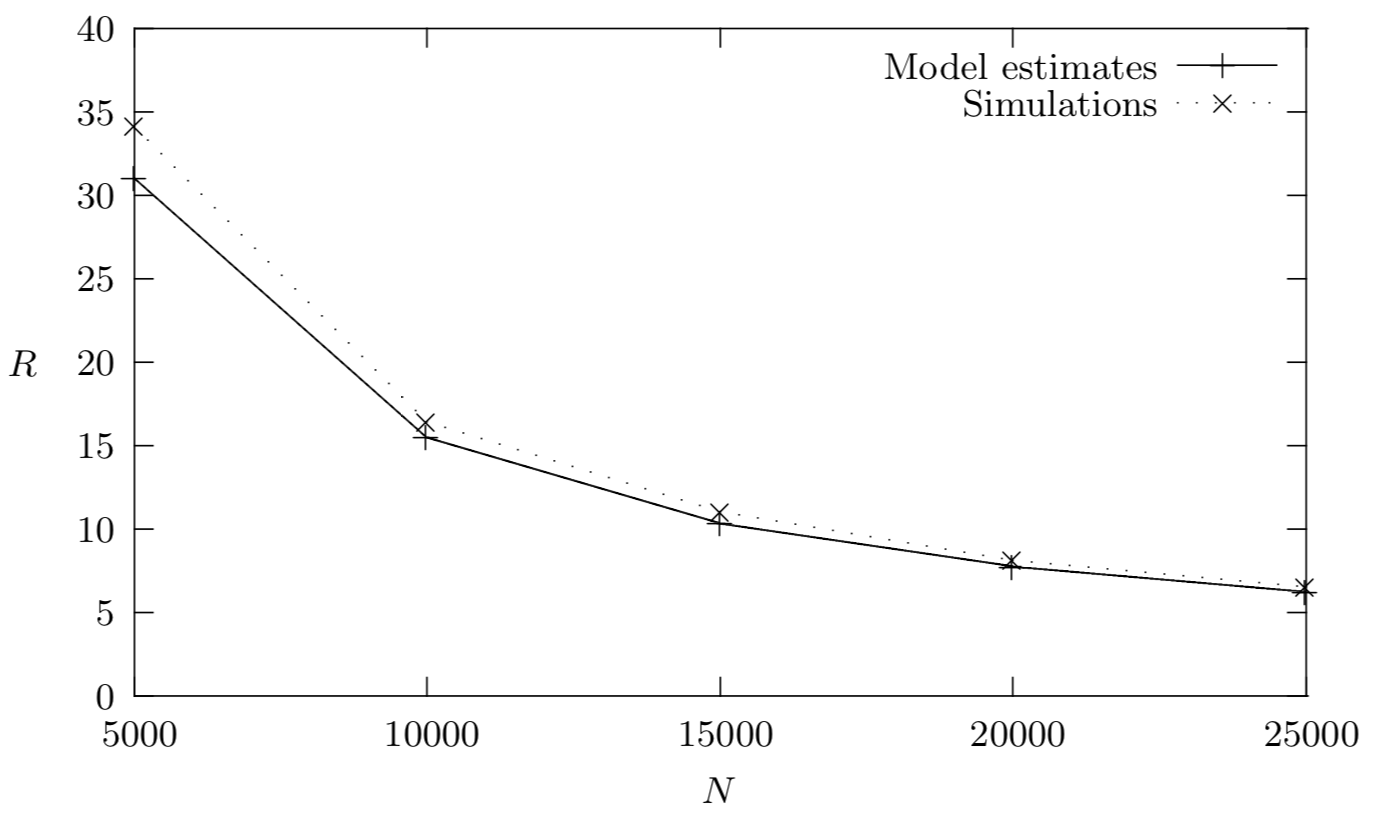
\includegraphics[scale=0.35]{images/varying_num_edges.png}
    \caption{TPS $= 1000$, av updates/tnx $= 5$, av arbiter service time $= 10ms$, av network delay $=5ms$}
  \end{figure}
\end{frame}

\begin{frame}
  \frametitle{Aborts per second $(\boldsymbol{R})$ vs Transaction Arrival Rate $(\boldsymbol{\lambda})$}
  \begin{center}
    Arbiter queue unstable at $\sim1500$ TPS
  \end{center}
  \begin{figure}[h!]
    \centering
    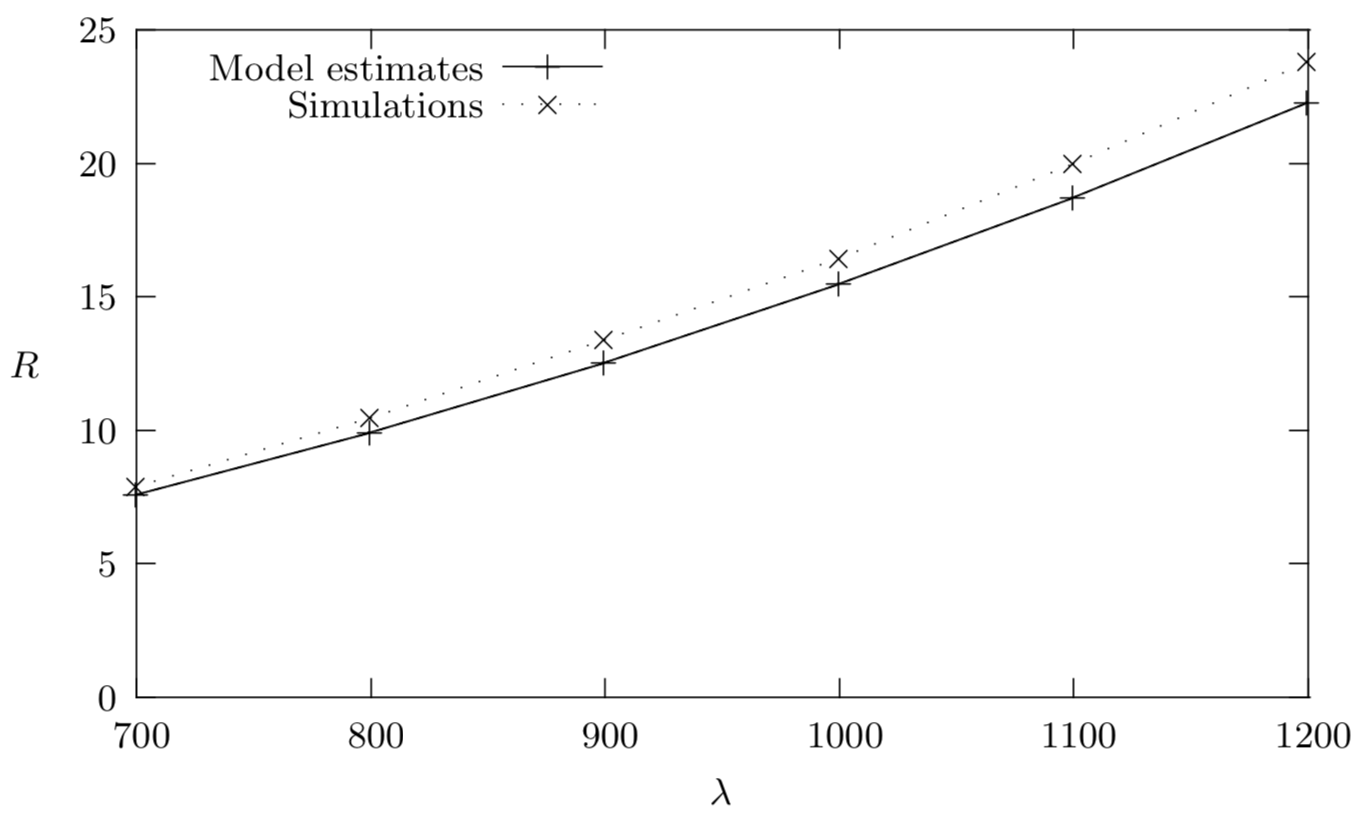
\includegraphics[scale=0.35]{images/varying_tnx_arrival_rate}
    \caption{\textcolor{red}{size $= 10K$}, av updates/tnx $= 5$, av arbiter service time $= 10ms$, av network delay $=5ms$}
  \end{figure}
\end{frame}

\begin{frame}
  \frametitle{Aborts per second $(\boldsymbol{R})$ vs Transaction Arrival Rate $(\boldsymbol{\lambda})$}
  \begin{center}
    Arbiter queue unstable at $\sim 1100$ TPS
  \end{center}
  \begin{figure}[h!]
    \centering
    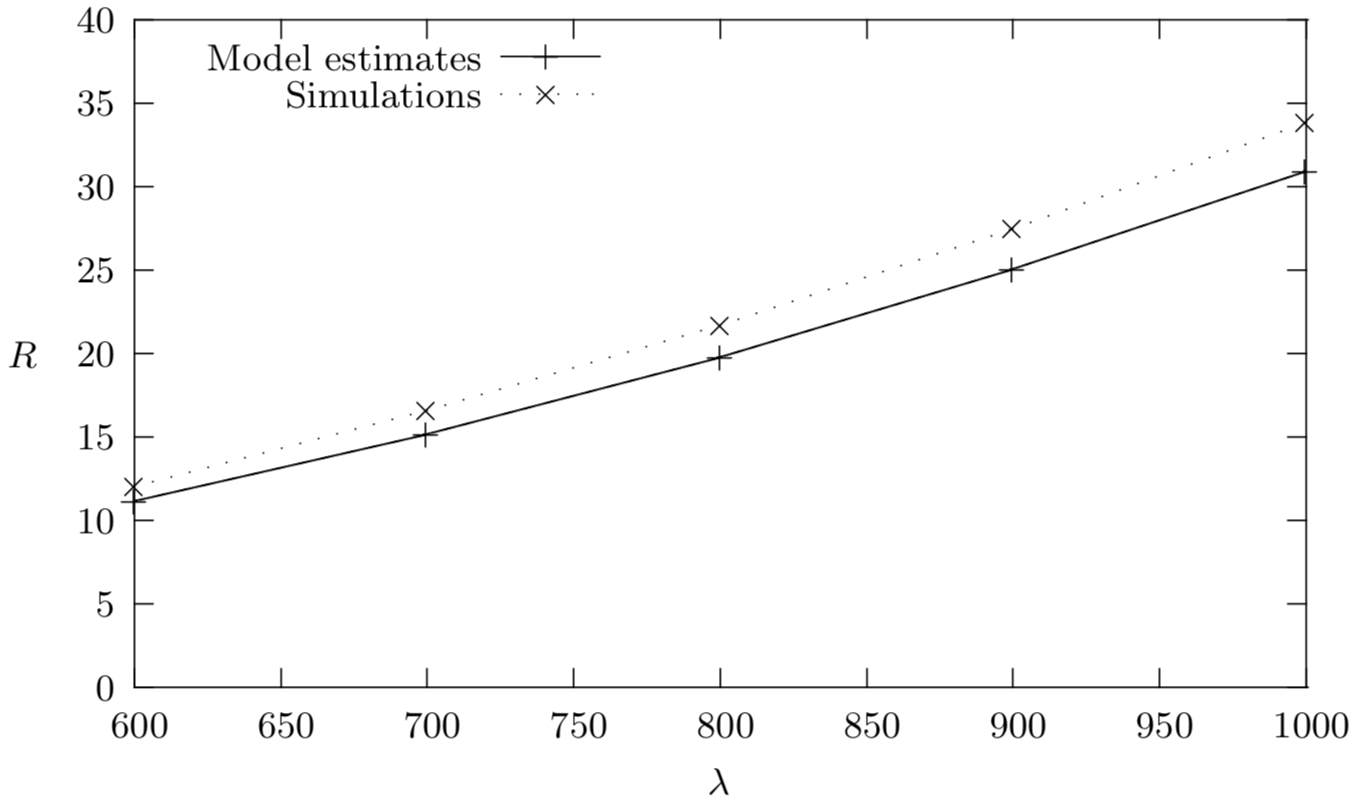
\includegraphics[scale=0.35]{images/larger_network_delay.png}
    \caption{size $= 10K$, av updates/tnx $= 5$, av arbiter service time $= 10ms$, \textcolor{red}{av network delay $=10ms$}}
  \end{figure}
\end{frame}

\begin{frame}
  \frametitle{Aborts per second $(\boldsymbol{R})$ vs Transaction Arrival Rate $(\boldsymbol{\lambda})$}
  \begin{center}
    Arbiter queue unstable at $\sim 550$ TPS
  \end{center}
    \begin{figure}[h!]
    \centering
    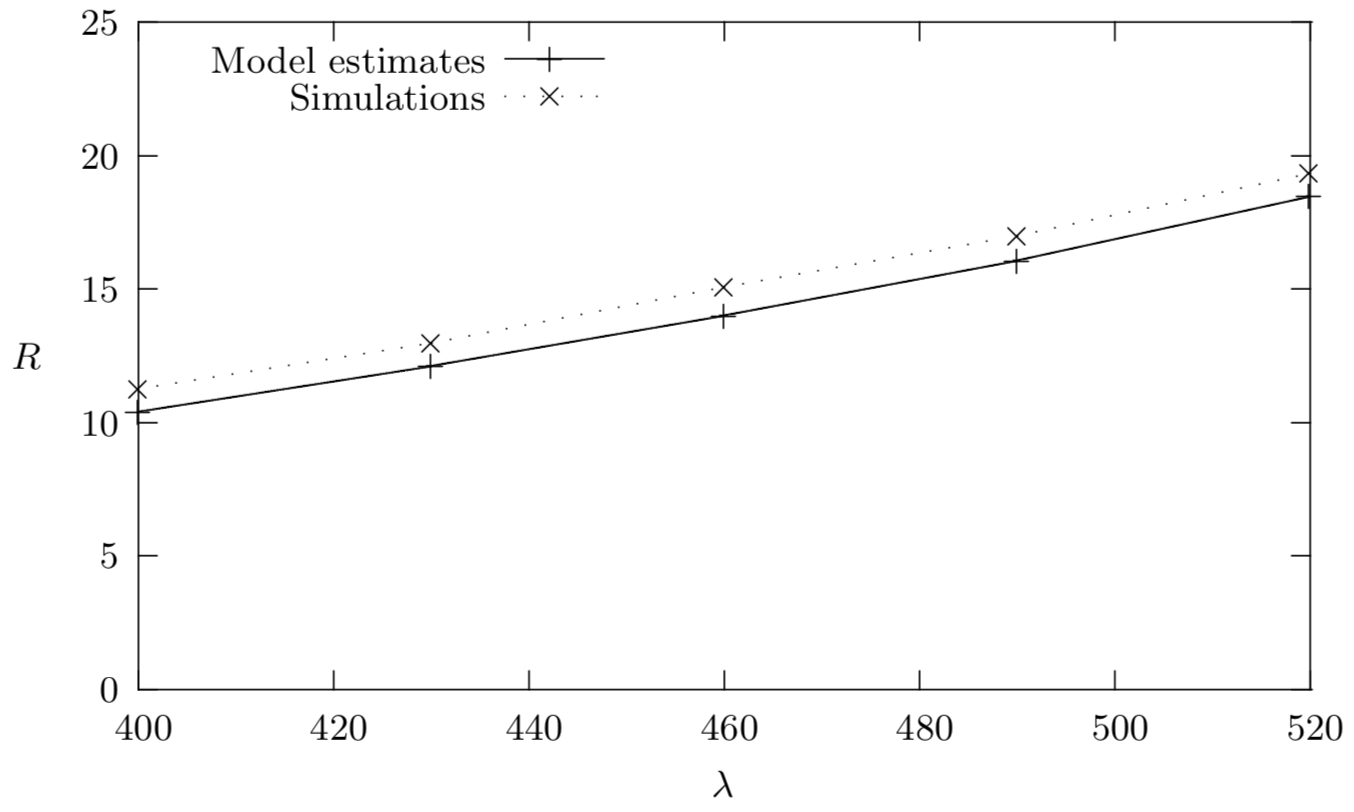
\includegraphics[scale=0.35]{images/varying_updates_per_tnx.png}
        \caption{size $= 10K$, \textcolor{red}{av updates/tnx $= 10$}, av arbiter service time $= 10ms$, av network delay $=5ms$}
  \end{figure}
\end{frame}

\begin{frame}
  \frametitle{Summary and Future Work}
  \begin{itemize}
    \uncover<1->{
    \item Model accuracy similar to simulations under a variety of parameter settings
    }
    \uncover<2->{
    \item Between 1-4\% transactions are aborted
    }
    \uncover<3->{
    \item Improve accuracy of simulation
    }
  \end{itemize}
\end{frame}

\begin{frame}[standout]
 Thanks for listening! \\
  \vspace{4mm}
  Any Questions? \\
  \vspace{4mm}
  {\normalsize Email: \href{mailto:j.waudby2@newcastle.ac.uk}{j.waudby2@newcastle.ac.uk}} \\
  {\normalsize Twitter: \href{https://twitter.com/waudberry_7}{@waudberry\_7}}
\end{frame}

\end{document}
